\documentclass[../main.tex]{subfiles}

\begin{document}

    In order to run hybrid continuous deployments, a \gls{hybrid_cloud} environment and a legacy stack have to be set up.
    An interactive script is available that is guiding through the setup (Fig.~\ref{fig:interactive_stetup}).

    \begin{figure}[h]
        \centering
        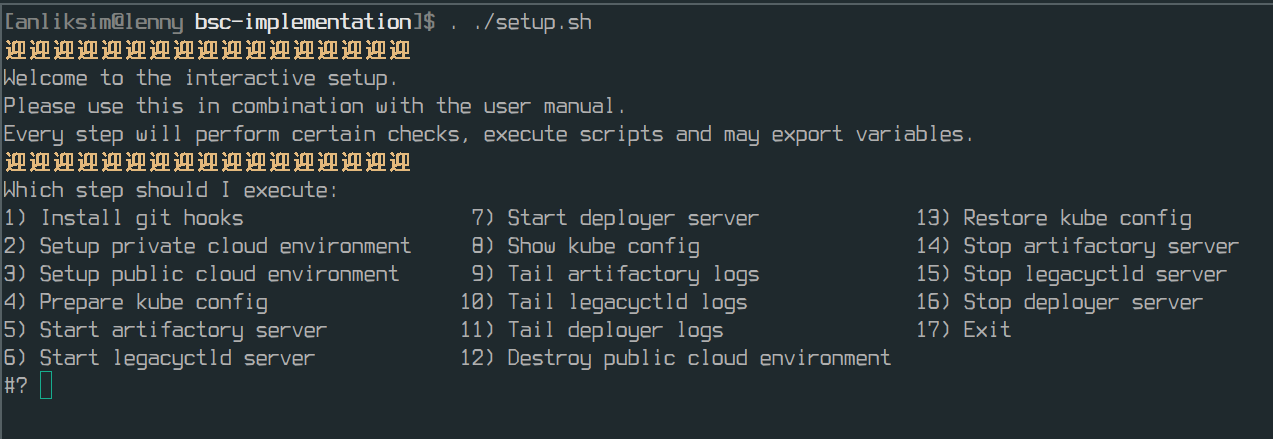
\includegraphics[width=\linewidth]{img/interactive_setup.png}
        \captionsetup{justification=centering}
        \caption{
            Interactive setup for hybrid continuous deployments with a hybrid cloud environment and a legacy stack.
        }
        \label{fig:interactive_stetup}
    \end{figure}

    First, checkout the implementation work using \gls{git}.

    Afterwards, the required steps are:
    \begin{itemize}
        \setlength\itemsep{0em}
        \item Installing a local \gls{git} commit hook on \verb|bsc-env|
        \item Setting up the \gls{private_cloud} environment locally with \gls{minikube}
        \item Setting up the \gls{public_cloud} environment on Microsoft \acrshort{aks} with \gls{terraform}
        \item Setting up the legacy stack locally
        \item Setting up the deployment workflow locally
        \item Setting up monitoring dashboards for \gls{grafana} with \gls{terraform}
    \end{itemize}

    A detailed user manual describing each step can be found as part of the \verb|bsc-implementation| at \verb|docs/manual.md|.

\end{document}

